
\section{Umělá inteligence(UI) - Definice, úzká UI obecná UI, superinteligence, strojové učení}
Umělá intelgince je výpočetní systém vykonávající činnost, kterou si spojujeme s lidskou inteligencí\\
Další definice: 
\begin{itemize}
    \item počítačové systémy, které jsou schopné plnit úkoly, které obvykle vyžadují lidskou inteligenci, jako je rozhodování, detekce objektů, řešení složitých problémů
    \item vědní disciplína, zabývající se teoríí systémů zpracovávajících data a schopných se víceméně samostatně rozhodovat
    \item schopnosti počítače/algoritmu napodobovat/realizovat některé funkce lidského mozku
\end{itemize}
\subsection*{Úzká umělá inteligence}
stupeň UI zahrnující stroje, které mohou provádět pouze úzce definovaou sadu konkrétních úkolů\\
jediná forma, které lidstvo doposud dosáhlo\\
aplikace na rutinních pracích - rozpoznávání řeči, obrazu, počítačové vidění, inteligentní budovy, hra šachů, návrh nákupu, počasí\\
UI je vznešený název pro sofistikované SW řešení, vkládáme důvěru do autora, že nic neopomenul\\
\begin{figure}[H]
    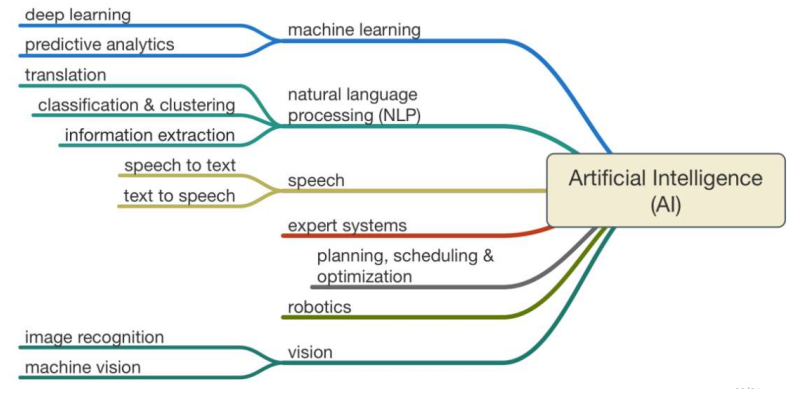
\includegraphics[scale = 1]{images/uzkeAI.png}
\end{figure}
\subsection*{Obecná UI}
Umělá inteligence na úrovni člověka\\
umí se rozhodovat, komunikovat, samostatně se učit\\
zatím není vyvinuta\\
Tuninguv test - nemožnost rozeznat člověka od stroje\\

\subsection*{Superinteligence}
má vyšší inteligenci než člověk\\
uvědomuje si, že ji ovládají a omezují intelektuálně podřadní lidé\\



\subsection*{Strojové učení(machine learning)}
\begin{itemize}
    \item zaměření na to, aby se stroje rozohodovaly na základě dat
    \item techniky strojového učení:
    \item \begin{itemize}
        \item učení s učitelem
        \item učení bez učitele
        \item zpětnovazební učení, posílené učení
    \end{itemize}
\end{itemize}
Učení s učitelem:
\begin{figure}[H]
    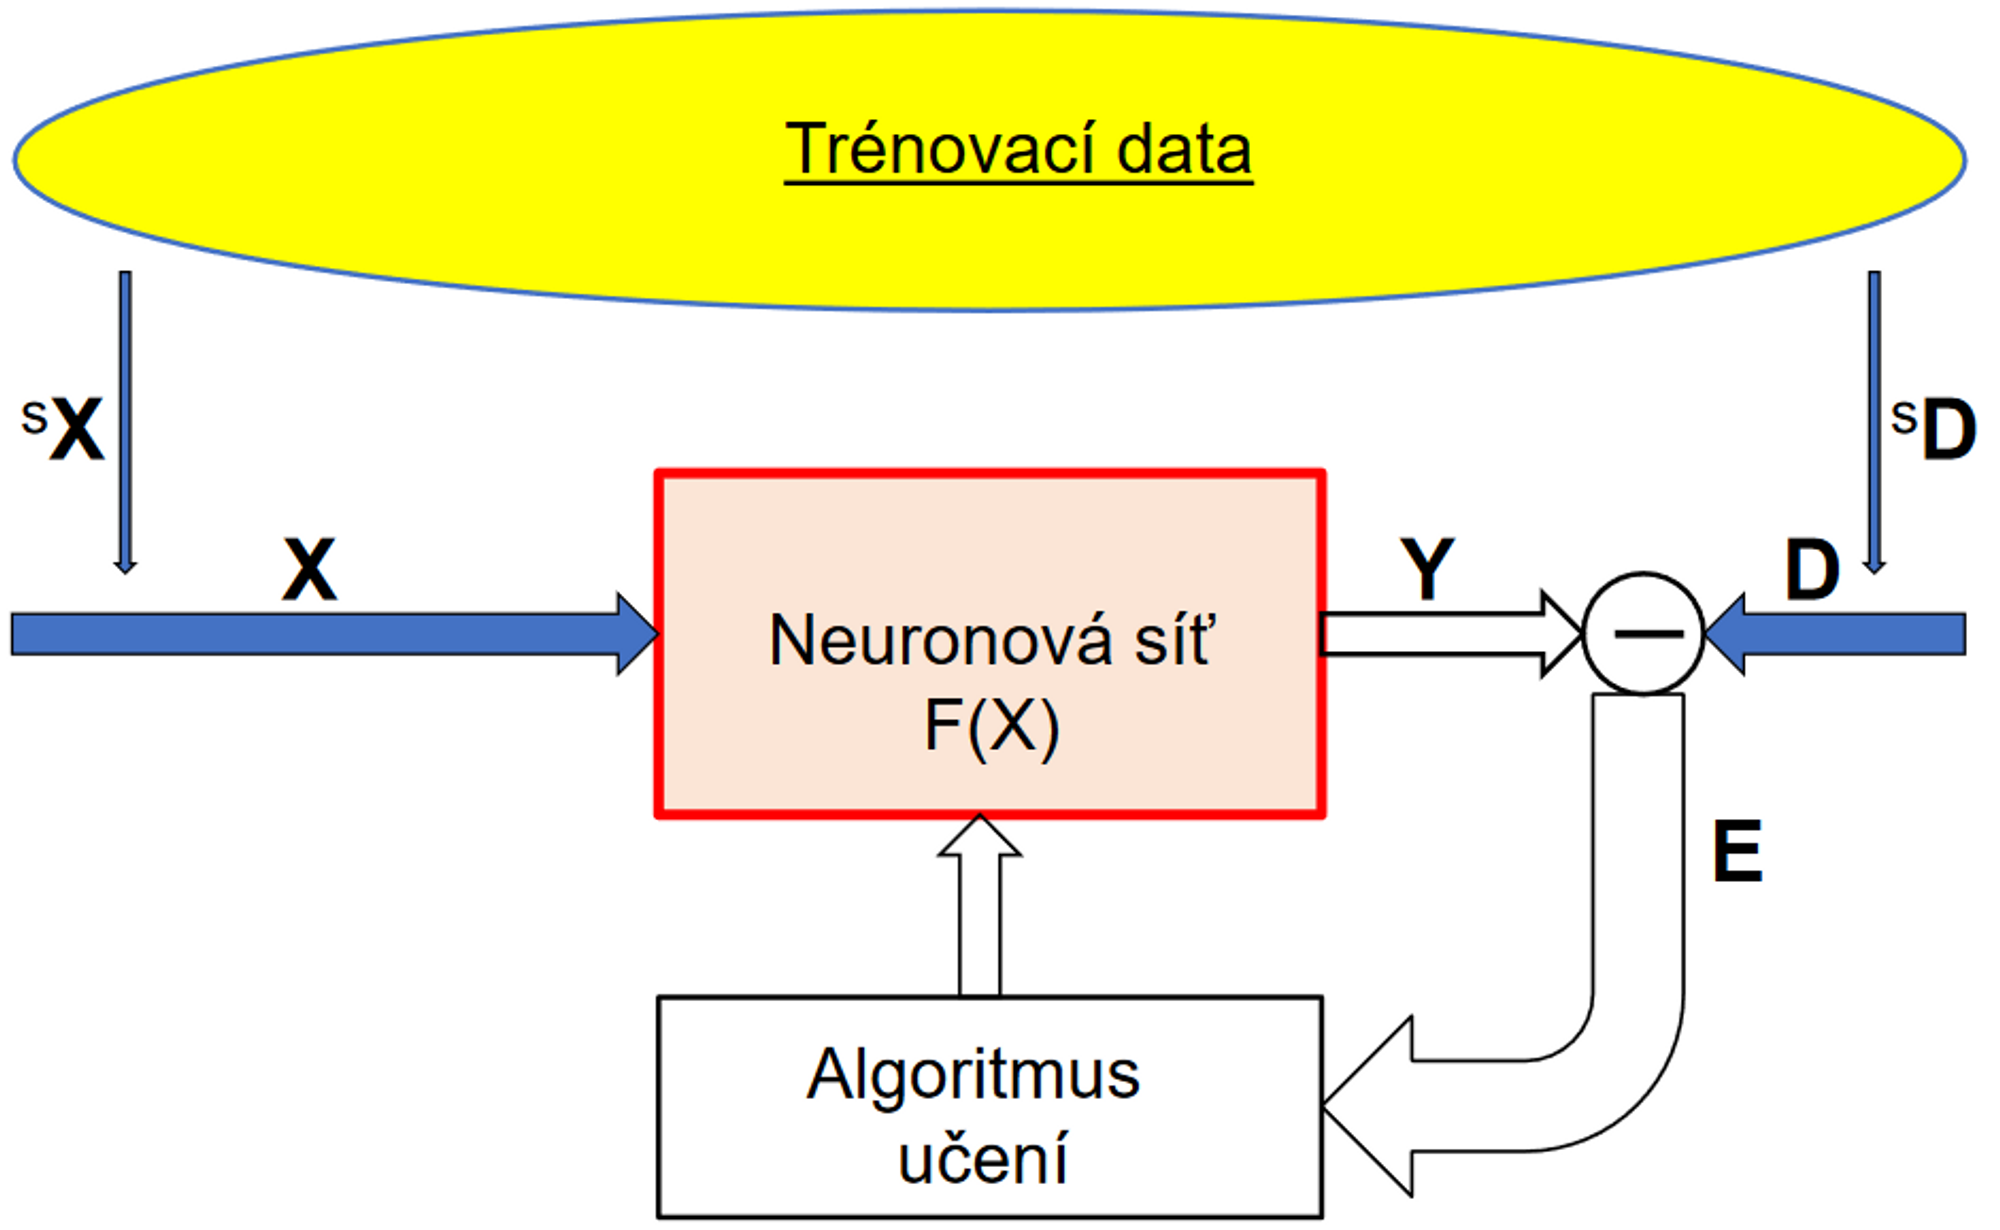
\includegraphics[scale = 0.3]{images/sUcitelem.png}
\end{figure}
Data jsou rozdělena na trénovací, validační a testovací\\
Učení probíhá tak, že systému předkládáme trénovací vzory a zároveň požadované výstupy, na základě kterých se mění váhy.\\
\newpage
Učení bez učitele:
\begin{figure}[H]
    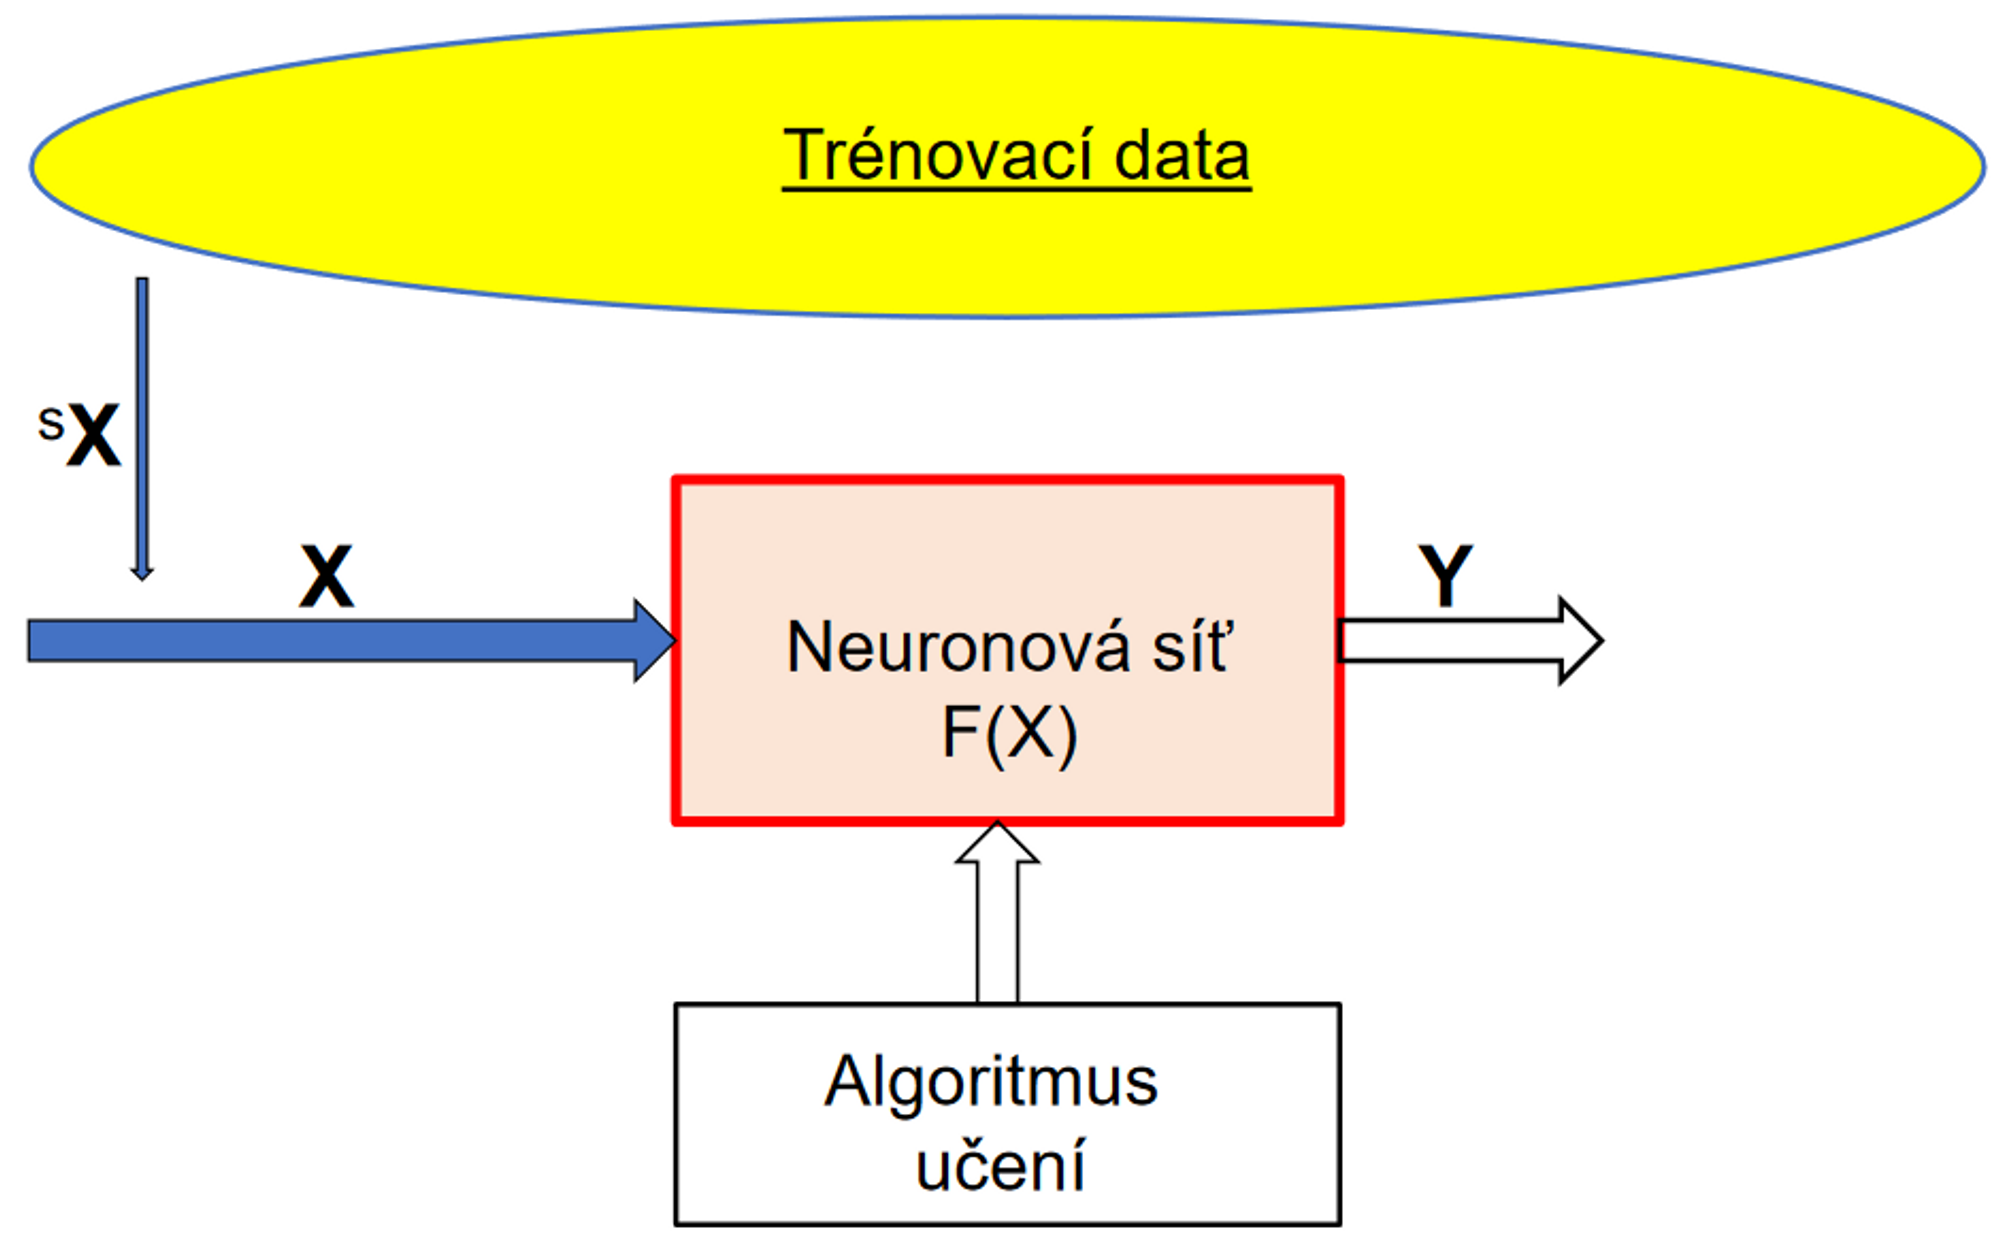
\includegraphics[scale = 0.4]{images/bezUcitele.png}
\end{figure}
Data jsou pouze jednoho typu a to trénovací\\
Učení probíhá tak, že jsou systému předloženy sady vstupů(bez správných výsledků, protože je neznáme) a na základě vstupů se mění váhy.\\

Existuje i kombinace obou přístupů, nazývá se expectation maximization algoritmus.

\subsection*{Základní druhy úloh}
\begin{itemize}
    \item Klasifikace vstupních dat do tříd
    \item Odhadování výstupní hodnoty podle vstupu
    \item Zařazování objektů do skupin podle podobných vlastností - učení bez učitele
\end{itemize}